\begin{center}
\section*{Annexe \uppercase\expandafter{\romannumeral 5} : Gestion de Maintenance Assistée par \hbox{Ordinateur} (GMAO) }
\addcontentsline{toc}{section}{Annexe \uppercase\expandafter{\romannumeral 5} : Gestion de Maintenance Assistée par Ordinateur (GMAO)}
\label{GMAO}
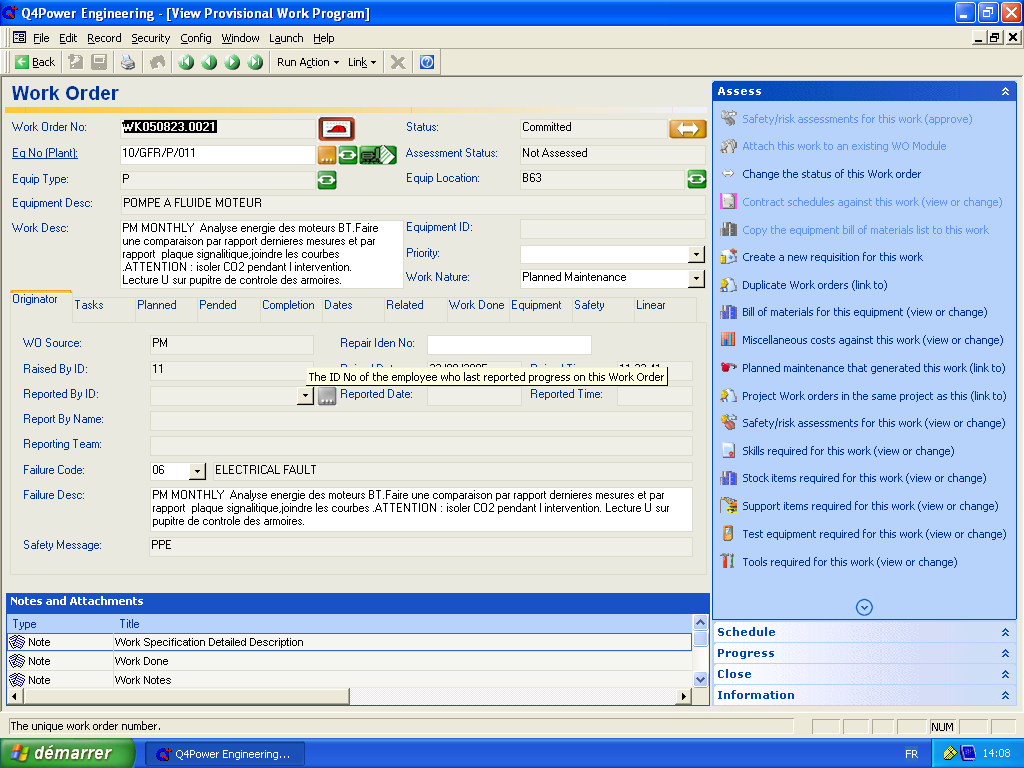
\includegraphics[scale=0.4]{./Figures/fenetre_travail_q4power.png}\vspace{10pt}
Session de Travail Engica
\end{center}
Pour les grandes sociétés, la planification manuelle des travaux de maintenance peut s'avérer une tâche pénible voir même impossible. \\C'est pourquoi, la centrale CPC opte pour une gestion automatisée. 

En effet, ses employés gèrent leurs travaux par un logiciel GMAO  ou CMMS (Computer rised Maintenans  Mangement System) nommé "Engica"(Q4). Ce logiciel offre plusieurs services notamment la possibilité  d'organiser les ressources, les programmes de maintenance et  les procédures dans un dépôt sûr.

 Les informations stockées peuvent être accédées par un dispositif de bureau, un navigateur web ou mobile. Chaque employé possède un compte accessible via un login et d'un mot de passe.
 
